\section{Introduction}
Most patients consult medical pratictioners when they fall sick with the aim of receiving treatment for that illness. Typically, on the first day of the treatment process, the doctor would analyze the symptoms that the patient's body is displaying, provide a diagnosis and finally prescribe the medication that is suitable to combat the patient's illness. For the rest of the treatment process (which could stretch to 4 weeks or more), it becomes the patient's responsiblity to heed the medical practioner's advice and follow the prescription suggested. Research has shown that not all patients follow their given prescription to the letter, some even experiencing recurring infections of the same disease they were treated initially treated for\cite{Vern01}. This reluctance to follow a medical prescription has been coined as non-adherence, implying that adherence is the ease at which patients follow a medical prescription\cite{Vern01}. There have been several studies published on medical adherence, the first of which dating back to 1968\cite{Fernerty12}. There are two common ways in which researchers have defined medical compliance. Frequently adherence is given the previously mentioned definition in that it is seen as the degree to which a patient follows a medical professional's drug prescriptions\cite{Vern01, Fernerty12}. Others choose to view compliance from a result perspective, whereby medical professionals measure a patient's compliance by evaluating the state of the patient's health. Another definition looks at the extent at which a patient's lifestyle changes in order to comply with a medical professional's prescription \cite{Vern01}. All of these definitions are primarily concerned about getting insights as to what happens after the doctor-patient consultation has been concluded, all the way through to the end of the medication treatment process.

Patients that incorrectly administer their medication are likely to fall sick again to the same illness and requiring additional medical resources for treatment\cite{Vern01, Kali99}. Avoidable instances such as these seek to undermine the level of healthcare that can be offered by the facility as the facility would undoubtedly incur costs in providing the same patient with more medication, medication that could have been efficiently dispensed to other patients that need them\cite{Vern01}. As a result, there has been a growing interest within the medical research fraternity to try and understand what would cause patients to not follow the prescriptions given by their medical practitioner. Researchers have looked into ways of improving doctor-patient consultations with the hope that patients have an increased appreciation of the importance of satisfying a medical practitioner's medical prescription.

The authors of this paper have chosen to focus on the medical prescriptions given out by doctors with furthur emphasis on the understanding the format these prescriptions could take when addressing patients who are not first language English speakers. We set out to acertain if there are any benefits to giving patients their medical prescriptions, through audio, in a language they are comfortable in, in this case isiXhosa. To evaluate if giving patients prescriptions in a local language would be beneficial, we sought out to test a patient's understanding of the prescription and how easily they could remember the contents of the prescription after 5 days. We also used an app to simulate and monitor a patient administering medication during the same period, with the aim of reporting on any benefits or setbacks on adherence. This paper has five sections, firstly its the introduction followed a furthur analysis presented by non-adherenceby previous research into adherence, followed by section 3 that details how the study was conducted then comes the results and discussion and finally the conclusion.


\section{Non-Adherence: Consequences and plausible causes}
\subsection{Implications}
\subsubsection{Financial}
Recurring illnesses result in extended treatment procedures which require additional provision of health care resources which are sometimes more costly\cite{SAGov16, Vern01}. This avoidable cost is incurred by both the facility and the patient. It is therefore especially problematic in resource limited settings which one would find in informal settlements such as townships in Cape Town, South Africa.

 \subsubsection{Health}

 Perhaps the most damaging consequence of non-compliance is its role in undermining the effect that the prescribed medication would have on the patient's wellbeing\cite{Vern01}. For instance, a patient that were to stop taking his/her medication may show the same symptoms after some time, suggesting that there might have been a resurgence of the same infection that she was given medical prescriptions for. This avoidable instance would mean that the patient's treatment process is delayed and furthur more the infection might have mutated  to become resistant to the initial prescription necesitating more complex (in some cases, more costly) prescription drugs. A real life scenario of this is with patients being treated for either tubercolosis or HIV. Without loss of generality, let us consider the case of TB. Patients diagnosed with TB are given prescription drugs to combat that infection but if the patient does not adhere, the infection or strain of TB can mutate to a more resistant strain called drug-resistant tubercolosis (DR-TB) or even worsen to multidrug-resistant tubercolosis (MR-TB) of which is a severe case and may be incurable \footnote{There exists strains of multidrug resistant tubercolosis that as of 20/09/2017 were deemed incurable}\cite{SAGov16}. Such chronic illnesses are especially problematic in countries such as South Africa, where the ministry of health released a report in 2016\cite{SAGov16}that states that the country has the third largest population of TB patients. The same report\cite{SAGov16} furthur estimates that by 2025 there could be a total of 12.3 million people suffering from chronic illnesses such as HIV and TB in that country.

\subsection{Causes}
Non-adherence to a medical professional's prescription can take on many forms. These could be (but not limited to) 1) a patient failing to follow medical professional's prescriptions (be it in terms of dosages, times of administering or prematurely stopping the medication), 2) delay in reporting illness and 3) missing appointments or follow up sessions\cite{Vern01}. Looking at the forms non-adherence can take can help in identify it's causes. Subsequently, researchers have suggested reasons to try and explain these causes. These suggestions include 1) increased complexity of drug prescriptions \cite{Fernerty12}, 2) health literacy of patients (combined with a general lack of confidence in medical professional)\cite{Kali99} and lastly high costs associated with accessing the medical treatment\cite{Vern01}. To add on to the last point, a study conducted by Verneire et al\cite{Vern01}, patients who did not come for follow up sessions cited transport costs as reason why they could not come as the health care facilities were often too far away from patients. Furthermore, expensive treatment artefacts or procedures were also cited as being reasons why some patients decided not to heed a doctor's prescription as they could not afford the treatment. To elaborate further on the second suggestion that researchers's made; researchers have found out that patients possesing a higher understanding of medicine were more likely to stop taking their medication often suspecting a misdiagnosis by the medical professional or a general lack of confidence in his/her abilities as a medical professional\cite{WilsonWolf}. For the first suggestion, complex medical prescriptions, will be the focus of this paper. Houts et al\cite{Houts06} have suggested that compliance to a medical prescription is due to 3 cognitive concepts, namely the ability to recall and understand a prescription and how much attention the patient placed on following the prescription. The solution suggested to the problem of adherence in this paper will focus on addressing these 3 aspects.


\section{Improving Doctor-Patient Communication}
As previously stated, non-adherence presents a serious challenge in South Africa. Here we propose a solution that addresses non-adherence by touching on 2 of the 3 cognitive concepts mentioned by Houts et al.
\subsection{Recall}
To improve the ease at which patients are able to remember their medical prescription, we follow the conclusion that Lester et al came to, in that short messages are more effective and easier to remember than long winded narrations. Secondly, through our system, we aim to make the prescription available to patients at anytime. This again is done to remind the patients what the prescription is, in the case the patient has forgotten, easing the cognitive load placed upon patients.
\subsection{Comprehension}
Currently, a number of patients in South Africa rely on labels written in English on their medication as their source of reference when they want to remind themselves of the medical prescription they have received from the medical professional. The use of English in these labels carries a heavy assumption in that the audience/patients are comfortable in that language, this is not always the case for residents of South Africa.Furthermore these labels have been criticized by medical researchers for being too complicated for people outside the medical fraternity to understand, citing the frequent use of medical jargon as the reason behind this\cite{Houts06}. To this end, Davis et al have been recommended that medical professionals should use vocabulary that is accessible to the patient because ultimately he/she will be the one reading the presctiption when taking in the medication.

To address all these shortfalls of the system, we suggest the use of an application that will disseminate these medical prescriptions as simple and concise narations in isiXhosa, a native language in South Africa. We hope, in this way, that patients can easily learn and fully understand the importance of following their given prescriptions. The use of audio to aid in learning presents some interesting promises especially when one considers the Mayer's cognitive theory of multimedia learning. In his writing, Mayer suggests that visual and verbal communication allows for a deeper understanding of the content being taught\cite{WilsonWolf}. Perhaps this can be explained by the fact that people have been consuming information through dialogues from child birth and so it is a learning technique that is not difficult to follow\cite{Patel10}.


\section{Related Work}
\subsection{Interventions and Adherence}
There have been a number of publications that looked at adherence. Most publications have focused on providing interventions during the treatment process by sending SMSes as reminders to patients to take in their medication\cite{Strand10, Lester10, Pop11}. All 3 studies, \cite{Strand10, Lester10, Pop11}, have seen varying increase in adherence rates but it remains to be seen if these interventions are economically feasible in resource limited settings in the longterm (well after their pilot phase). Furthermore, we believe there could be an added benefit of providing prescriptions through the use of audio as it could help patients better understand the medication. Another intervention study by Forster et al \cite{Forster08} examined the use of electronic medical record (EMR) systems in identifying HIV patients that are more likely to be non compliant. Patients who missed follow up appointments were identified in a timely manner so as to initiate the intervention strategies to boost adherence. The study does not have a conclusive answer as to whether or not the use of EMR systems does indeed increase adherence. This is partly due to the fact the EMR systems are not the actual intervention strategy but aid other strategies. The only conclusion that the researchers could draw was that more missing data often lead to more patients failing to attend appointments.

\subsection{Prescriptions and Adherence}
Verneire et al \cite{Vern01} have emphasized the need for medical professionals to help patients understand the prescription and as such have advocated for a more in depth analysis of the cognitive factors that play a role in a patient's adherence to the prescription. In \cite{Ostini14} researchers point out that a non-adherent patient that does not possess a high health literacy is more likely to cite forgetfulness rather than citing a lack of confidence in the medication or the medical professional as the reason why he or she took an incorrect dosage of the medication, in both cases supporting Verneire et al's earlier statements. In this vain, Davies et al \cite{Davis06} have looked at simplifying prescriptions labels through the use of pictorial aids and simpler language, they concluded that there are benefits to this as patients showed a clearer understanding of the contents of the prescription.

\subsubsection{Audio and Learning}
Audio systems have been the preferred medium of communication especially in developing communities. A successful example of this is the use of relayed audio messages in the Avaaj Otalo paper published by Patel et al \cite{Patel10}, where by the researchers setup a system that connected farmers in a rural region of India. The farmers were encouraged to pose questions and listen to responses from other farmers or listening to other professionals who could be giving out farming advice on the platform. The system showed signs of success in its phase even being used to share other community news. Although the researchers did not evaluate how much was learnt through the system, a number of users reported to have gained some form of education through the system be it about farming techniques or how to control pests. The same is true for other IVR services, like SpokenWeb \cite{Spoken10}, dispensing educational material through the use of audio, there is little emphasis placed on evaluating the learning impact of providing such systems to people.
An interesting study by Ramkrishnan et al\cite{DocTalk} has also decided to give patients access their medical prescriptions through voice recordings recorded by the patient's doctor. Unfortunately, the adoption of this system was poor with the authors citing the doctor's busy schedule as the main culprit. As such, they could not conduct experiments to report on potential benefits to audio systems in the medical fraternity. However, Joshi et al \cite{Joshi13} designed an intervention strategy, that makes use of an audio system to give out 'treatment advice' to people living with HIV and AIDS, and have since reported it to have a 'desired effect' on adherence rates. The system makes us of voice calls to patients to remind them about their medication, it also provides the patients with a voice driven interface where users can report any further symptoms that they could be displaying, or listen to upcoming appointments or health tips. This system would work well in the South African context, had it not been for the cost implications associated with voice calls and the fact that it relies heavily on good internet access at hospitals to work.

To this end, we have designed a system, similar to both the works of Joshi et al \cite{Joshi13} and Ramkrishnan et al\cite{DocTalk}. Similar to TAMA (TREATMENT ADVICE BY MOBILE ALERTS by Joshi et al) in that it also gives out medical prescriptions and monitors usage. And also, similar to DocTalk by Ramkrishan et al in that it uses voice recordings that can be played locally on the phone.


\section{Study}
\subsection{Overview and Research Question}
In this study we hoped to answer 2 research questions; 1) are there any benefits to adherence when patients are given medical prescriptions through audio in a native language that is not English, like isiXhosa, and secondly does the use of audio help patients recall and understand their prescriptions? This study is part of a larger study that looks at if there's any significant difference in adherence rates in giving patients their medical prescriptions in the local langauge and which mode (auido, text or through pictures) shows the most promise. To help answer all these questions, we set out to give patients their medical prescriptions in isiXhosa using audio recordings and monitor how they take their medication. Monitoring how they take their medication helps us answer questions around adherence. To answer questions around recall and comprehension we asked participants some open ended questions to test how easy they could remember the contents of their prescription and to see if they had indeed understood, with clarity, the contents and implications of the given prescriptions. It is worthnoting that this is not a clinical trial and as such we did not use actual patients but rather we asked isiXhosa speaking individuals to be part of the study. As this is not a clinical study, we used an app to simulate the process of a patient taking in medication, this is explained in more detail in Software Development section. The study was set out to start with a briefing session where we explained to the participants what the study is about and how we would go about conducting it. The patients/participants of the study then used the app for the next 5 days then returned after for a debrief session where we asked them questions to evaluate if they understood their prescriptions.

\subsection{Study Design}
\subsubsection{Participants}
We selected participants that were not only fluent in isiXhosa but were also comfortable in reading the language, reason being we did not want participants to favour one mode over the other (audio over reading) and introducing bias into the study. It was established that we were more likely to find such participants amongst the older isiXhosa speaking population as they are less frequently thwarted into scenarios requiring them to consume knowledge or interact in English, which is not the case with university students who learn primarily through English literature. And so we hoped to engage with the staff at the University of Cape Town (UCT) because we could easily access them but we were not able to secure the ethical clearance to do so in a timely fashion. Alas, we looked for participants from outside UCT, we talked to people that worked in shops, fuel refill stations, churchgoers after service and security guards. After talking to more than 25 people, we were able to successfully convince at least 12 people to be part of the study. Because of the nature of their work, we could not find a common time when everyone was free, and so we had to hold individual sessions, some would come in twos but mostly each participant came to the debrief session alone. To make sure that we give all participants the same information during the breifing session, we wrote a script of how the session would be conducted. Thus, the only difference in the information participants got would be through questions that each posed during the briefing session. These participants were split into two groups; control and the ones that received the audio treatment. This ended up being 2 groups of 5 as 2 participants did not return for the debrief session.

\subsection{Prescription}
In coming up with the prescriptions, we used the findings of a paper published by Berry et al \cite{Berry} where by the researchers ran 3 studies to determine what should the contents of a prescription include. In that study, Berry et al concluded that for a prescription to be considered sufficient, it should at least address 3 issues. Firstly, what is the medication for, secondly what are the side effects and finally what are the lifestyle changes that the patient should implement in order for him/her to experience the full benefits of the medication.
We fabricated a prescription for back pain. We intentionally chose not to use a known prescription because we did not want any participant recognizing the prescription and thus coming in with prior knowledge into the study which could skew our results. We wanted each participant to receive this relatively new information and be evaluated in the same manner. Both groups were given the same prescription, but in different formats. The control group was given the prescription through a pillcard that resembled the pillcards being given to patients in South African hospitals. It is worth noting that these are often in English and as such we gave our control group pillcards containing their prescriptions written in English. For the audio group, the prescription was recorded in isiXhosa the uploaded on a cloud database, firebase\footnote{Firebase is google's realtime database engine for mobile apps - https://firebase.google.com/}. In accordance with the recommendation of Davis et al, we made tried to make the recording as clear and concise as possible. keeping the record under 2 mins without leaving out any crucial information. We went a step further to record the 3 different sections that Berry et al mentioned in his paper separately; thus there was a recording explaining what the medication is for and how to administer it, there was a recording on what are the possible side effects and there weas a recrding explaining the lifestyle changes.

\subsubsection{Software Development}
As we have previously mentioned this is not a clinical study, therefore meaning that we did not give patients any real medication. To help us monitor adherence rates, we designed a mobile app that simulates the process of taking in medication. The idea was that patients would push a button and that would represent them taking their medication. For instance, if a patient is to take 3 pills at night, we would expect the participant to push the button 3 times. Additionally, we added a button that displays a screen where the patient can then listen to their prescriptions, but that was a button only available to the audio group as the control group had their prescription through their pillcard. The two screens for audio are shown below.

\begin{figure}
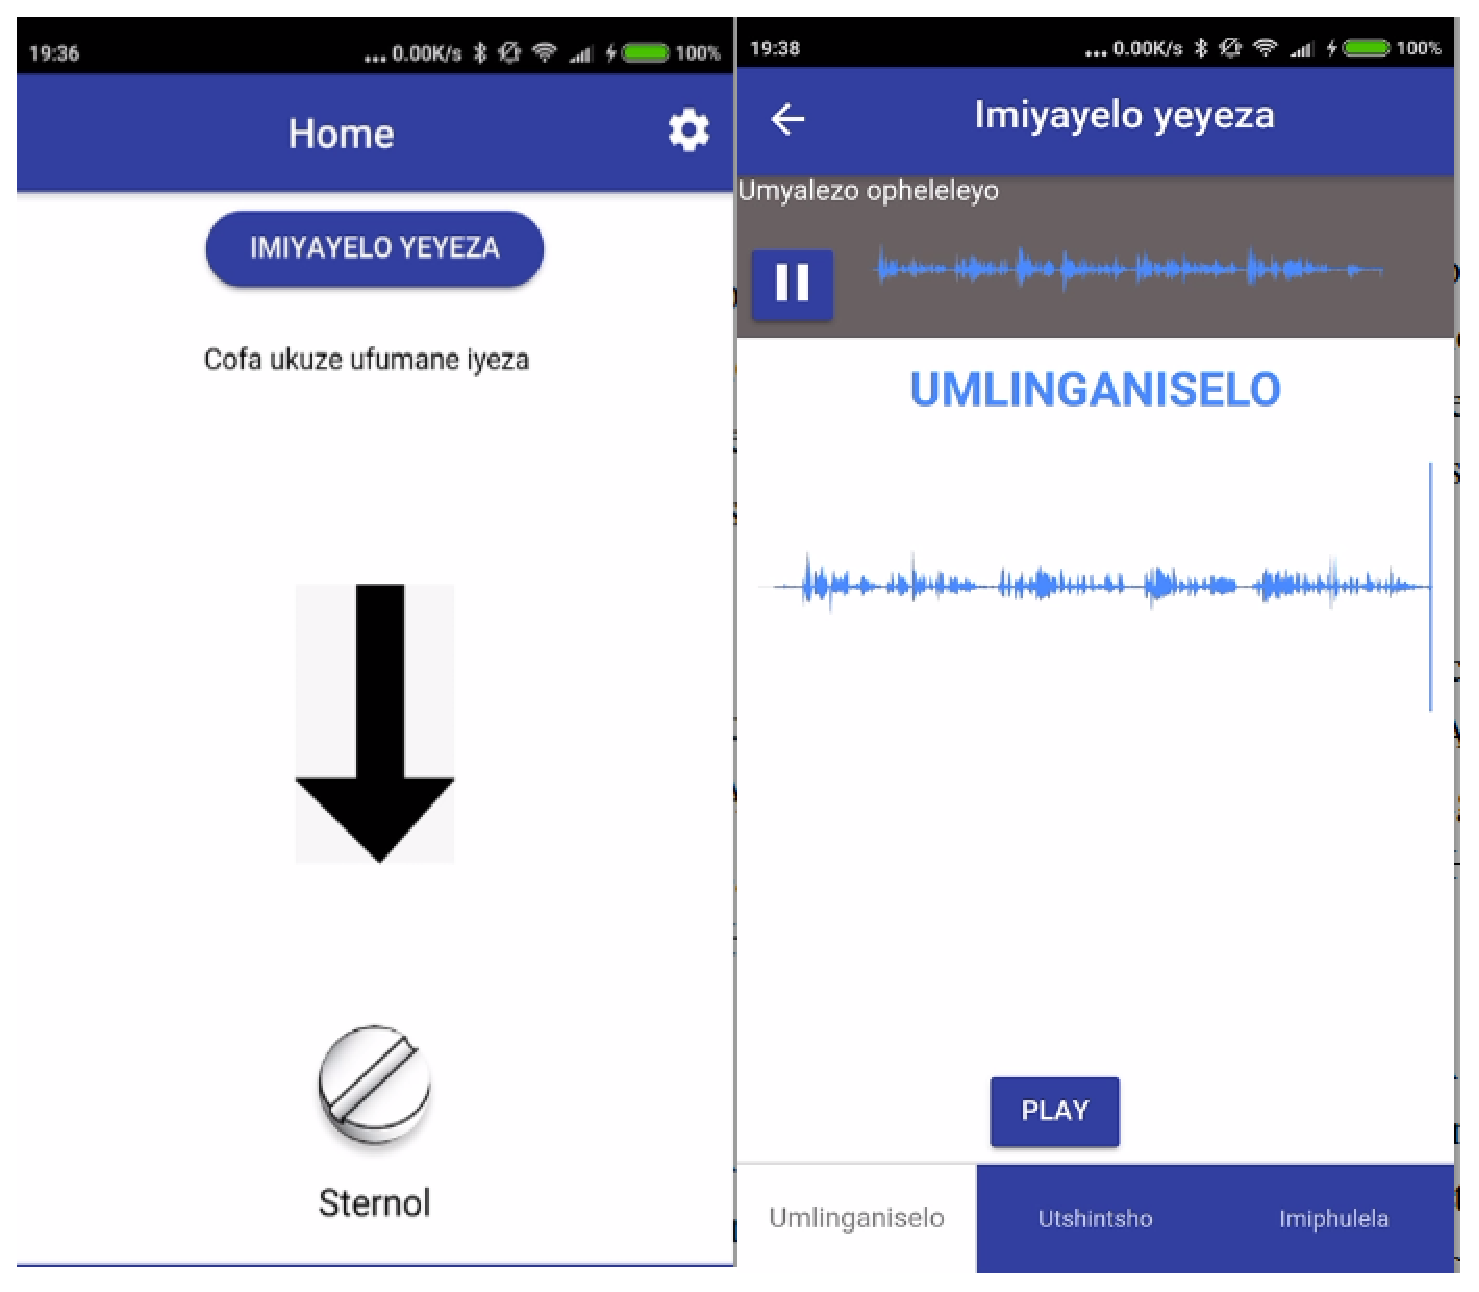
\includegraphics[width=\linewidth, height=200pt]{mobileapp}
\caption{A sceenshot of the home screen and the listening screen}
\end{figure}

To develop this app we used the ionic\footnote{Ionic 4 - ionicframework.com}, which allowed for us to develop a hybrid app that can be used across multiple platforms, or so we had hoped. Eventually it turned out that the version of ionic, version 4, we were using is not compatible with windows mobile phones and
due to financial constraints we could not compile an iOS\footnote{The operating system running on Apple phones, https://www.apple.com/za/ios/ios-10/} compatible version of the software\footnote{To write Apple apps one must have an apple console, to register an apple console one must register through their Apple Development Programme of which has a registration fee of 99USD}. Alas we had an android app, fortunately most of our participants had android phones. Ionic uses a webview\footnote{cordova - cordova.apache.org} as a wrapper to display all its components. It therefore allows developers to write mobile apps using web development tools such as AngularJS, HTML5 and SCSS to name a few, also one can use other javascript plugins that they deem necessary, as one does in web development. In fact, we did also use a number of opensource javascript plugins, like angularfire2\footnote{A plugin to connect your ionic v4 app to your firebase database and cloud storage - we used version 4.0.0-rc.2}.

For our database, we setup 13 separate users, 6 users for each group and a test user used during development. Firebase is a NoSQL database meaning all users were essentially a key-value pair where the user is the key and the value represents a collection of attributes for each user. These attributes helped us keep track of which users were already assigned and which prescription they were meant to on.

Participants were given the app through an app called ShareIt. After installing, the participants had to be assigned to the already populated user list in the database, at this time it did not matter much which user they were set to because there is only one prescription but since this is part of an ongoing study we might decide to have other users listen to different medical prescriptions, therefore needing the prescription variable to be dynamic. When the user is set, the prescription is read of that user profile and the corresponding audio files were downloaded from our firebase storage server. These files will sit locally on the phone, henceforth allowing the participant to play back the recordings without incuring any data costs.

Lastly the app is recording the time and date when a user presses on the button to take the medication.

% Typically, the body of a paper is organized into a hierarchical
% structure, with numbered or unnumbered headings for sections,
% subsections, sub-subsections, and even smaller sections.  The command
% \texttt{{\char'134}section} that precedes this paragraph is part of
% such a hierarchy.\footnote{This is a footnote.} \LaTeX\ handles the
% numbering and placement of these headings for you, when you use the
% appropriate heading commands around the titles of the headings.  If
% you want a sub-subsection or smaller part to be unnumbered in your
% output, simply append an asterisk to the command name.  Examples of
% both numbered and unnumbered headings will appear throughout the
% balance of this sample document.
%
% Because the entire article is contained in the \textbf{document}
% environment, you can indicate the start of a new paragraph with a
% blank line in your input file; that is why this sentence forms a
% separate paragraph.
%
% \subsection{Type Changes and {\itshape Special} Characters}
%
% We have already seen several typeface changes in this sample.  You can
% indicate italicized words or phrases in your text with the command
% \texttt{{\char'134}textit}; emboldening with the command
% \texttt{{\char'134}textbf} and typewriter-style (for instance, for
% computer code) with \texttt{{\char'134}texttt}.  But remember, you do
% not have to indicate typestyle changes when such changes are part of
% the \textit{structural} elements of your article; for instance, the
% heading of this subsection will be in a sans serif\footnote{Another
%   footnote here.  Let's make this a rather long one to see how it
%   looks.} typeface, but that is handled by the document class file.
% Take care with the use of\footnote{Another footnote.}  the
% curly braces in typeface changes; they mark the beginning and end of
% the text that is to be in the different typeface.
%
% You can use whatever symbols, accented characters, or non-English
% characters you need anywhere in your document; you can find a complete
% list of what is available in the \textit{\LaTeX\ User's Guide}
% \cite{Lamport:LaTeX}.
%
% \subsection{Math Equations}
% You may want to display math equations in three distinct styles:
% inline, numbered or non-numbered display.  Each of
% the three are discussed in the next sections.
%
% \subsubsection{Inline (In-text) Equations}
% A formula that appears in the running text is called an
% inline or in-text formula.  It is produced by the
% \textbf{math} environment, which can be
% invoked with the usual \texttt{{\char'134}begin\,\ldots{\char'134}end}
% construction or with the short form \texttt{\$\,\ldots\$}. You
% can use any of the symbols and structures,
% from $\alpha$ to $\omega$, available in
% \LaTeX~\cite{Lamport:LaTeX}; this section will simply show a
% few examples of in-text equations in context. Notice how
% this equation:
% \begin{math}
%   \lim_{n\rightarrow \infty}x=0
% \end{math},
% set here in in-line math style, looks slightly different when
% set in display style.  (See next section).
%
% \subsubsection{Display Equations}
% A numbered display equation---one set off by vertical space from the
% text and centered horizontally---is produced by the \textbf{equation}
% environment. An unnumbered display equation is produced by the
% \textbf{displaymath} environment.
%
% Again, in either environment, you can use any of the symbols
% and structures available in \LaTeX\@; this section will just
% give a couple of examples of display equations in context.
% First, consider the equation, shown as an inline equation above:
% \begin{equation}
%   \lim_{n\rightarrow \infty}x=0
% \end{equation}
% Notice how it is formatted somewhat differently in
% the \textbf{displaymath}
% environment.  Now, we'll enter an unnumbered equation:
% \begin{displaymath}
%   \sum_{i=0}^{\infty} x + 1
% \end{displaymath}
% and follow it with another numbered equation:
% \begin{equation}
%   \sum_{i=0}^{\infty}x_i=\int_{0}^{\pi+2} f
% \end{equation}
% just to demonstrate \LaTeX's able handling of numbering.
%
% \subsection{Citations}
% Citations to articles~\cite{bowman:reasoning,
% clark:pct, braams:babel, herlihy:methodology},
% conference proceedings~\cite{clark:pct} or maybe
% books \cite{Lamport:LaTeX, salas:calculus} listed
% in the Bibliography section of your
% article will occur throughout the text of your article.
% You should use BibTeX to automatically produce this bibliography;
% you simply need to insert one of several citation commands with
% a key of the item cited in the proper location in
% the \texttt{.tex} file~\cite{Lamport:LaTeX}.
% The key is a short reference you invent to uniquely
% identify each work; in this sample document, the key is
% the first author's surname and a
% word from the title.  This identifying key is included
% with each item in the \texttt{.bib} file for your article.
%
% The details of the construction of the \texttt{.bib} file
% are beyond the scope of this sample document, but more
% information can be found in the \textit{Author's Guide},
% and exhaustive details in the \textit{\LaTeX\ User's
% Guide} by Lamport~\shortcite{Lamport:LaTeX}.
%
% This article shows only the plainest form
% of the citation command, using \texttt{{\char'134}cite}.
%
% Some examples.  A paginated journal article \cite{Abril07}, an enumerated
% journal article \cite{Cohen07}, a reference to an entire issue \cite{JCohen96},
% a monograph (whole book) \cite{Kosiur01}, a monograph/whole book in a series (see 2a in spec. document)
% \cite{Harel79}, a divisible-book such as an anthology or compilation \cite{Editor00}
% followed by the same example, however we only output the series if the volume number is given
% \cite{Editor00a} (so Editor00a's series should NOT be present since it has no vol. no.),
% a chapter in a divisible book \cite{Spector90}, a chapter in a divisible book
% in a series \cite{Douglass98}, a multi-volume work as book \cite{Knuth97},
% an article in a proceedings (of a conference, symposium, workshop for example)
% (paginated proceedings article) \cite{Andler79}, a proceedings article
% with all possible elements \cite{Smith10}, an example of an enumerated
% proceedings article \cite{VanGundy07},
% an informally published work \cite{Harel78}, a doctoral dissertation \cite{Clarkson85},
% a master's thesis: \cite{anisi03}, an online document / world wide web
% resource \cite{Thornburg01, Ablamowicz07, Poker06}, a video game (Case 1) \cite{Obama08} and (Case 2) \cite{Novak03}
% and \cite{Lee05} and (Case 3) a patent \cite{JoeScientist001},
% work accepted for publication \cite{rous08}, 'YYYYb'-test for prolific author
% \cite{SaeediMEJ10} and \cite{SaeediJETC10}. Other cites might contain
% 'duplicate' DOI and URLs (some SIAM articles) \cite{Kirschmer:2010:AEI:1958016.1958018}.
% Boris / Barbara Beeton: multi-volume works as books
% \cite{MR781536} and \cite{MR781537}.
%
% A couple of citations with DOIs: \cite{2004:ITE:1009386.1010128,
%   Kirschmer:2010:AEI:1958016.1958018}.
%
% Online citations: \cite{TUGInstmem, Thornburg01, CTANacmart}.
%
%
% \subsection{Tables}
% Because tables cannot be split across pages, the best
% placement for them is typically the top of the page
% nearest their initial cite.  To
% ensure this proper ``floating'' placement of tables, use the
% environment \textbf{table} to enclose the table's contents and
% the table caption.  The contents of the table itself must go
% in the \textbf{tabular} environment, to
% be aligned properly in rows and columns, with the desired
% horizontal and vertical rules.  Again, detailed instructions
% on \textbf{tabular} material
% are found in the \textit{\LaTeX\ User's Guide}.
%
% Immediately following this sentence is the point at which
% Table~\ref{tab:freq} is included in the input file; compare the
% placement of the table here with the table in the printed
% output of this document.
%
% \begin{table}
%   \caption{Frequency of Special Characters}
%   \label{tab:freq}
%   \begin{tabular}{ccl}
%     \toprule
%     Non-English or Math&Frequency&Comments\\
%     \midrule
%     \O & 1 in 1,000& For Swedish names\\
%     $\pi$ & 1 in 5& Common in math\\
%     \$ & 4 in 5 & Used in business\\
%     $\Psi^2_1$ & 1 in 40,000& Unexplained usage\\
%   \bottomrule
% \end{tabular}
% \end{table}
%
% To set a wider table, which takes up the whole width of the page's
% live area, use the environment \textbf{table*} to enclose the table's
% contents and the table caption.  As with a single-column table, this
% wide table will ``float'' to a location deemed more desirable.
% Immediately following this sentence is the point at which
% Table~\ref{tab:commands} is included in the input file; again, it is
% instructive to compare the placement of the table here with the table
% in the printed output of this document.
%
%
% \begin{table*}
%   \caption{Some Typical Commands}
%   \label{tab:commands}
%   \begin{tabular}{ccl}
%     \toprule
%     Command &A Number & Comments\\
%     \midrule
%     \texttt{{\char'134}author} & 100& Author \\
%     \texttt{{\char'134}table}& 300 & For tables\\
%     \texttt{{\char'134}table*}& 400& For wider tables\\
%     \bottomrule
%   \end{tabular}
% \end{table*}
% % end the environment with {table*}, NOTE not {table}!
%
% It is strongly recommended to use the package booktabs~\cite{Fear05}
% and follow its main principles of typography with respect to tables:
% \begin{enumerate}
% \item Never, ever use vertical rules.
% \item Never use double rules.
% \end{enumerate}
% It is also a good idea not to overuse horizontal rules.
%
%
% \subsection{Figures}
%
% Like tables, figures cannot be split across pages; the best placement
% for them is typically the top or the bottom of the page nearest their
% initial cite.  To ensure this proper ``floating'' placement of
% figures, use the environment \textbf{figure} to enclose the figure and
% its caption.
%
% This sample document contains examples of \texttt{.eps} files to be
% displayable with \LaTeX.  If you work with pdf\LaTeX, use files in the
% \texttt{.pdf} format.  Note that most modern \TeX\ systems will convert
% \texttt{.eps} to \texttt{.pdf} for you on the fly.  More details on
% each of these are found in the \textit{Author's Guide}.
%
% \begin{figure}
% 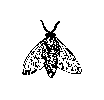
\includegraphics{fly}
% \caption{A sample black and white graphic.}
% \end{figure}
%
% \begin{figure}
% 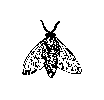
\includegraphics[height=1in, width=1in]{fly}
% \caption{A sample black and white graphic
% that has been resized with the \texttt{includegraphics} command.}
% \end{figure}
%
%
% As was the case with tables, you may want a figure that spans two
% columns.  To do this, and still to ensure proper ``floating''
% placement of tables, use the environment \textbf{figure*} to enclose
% the figure and its caption.  And don't forget to end the environment
% with \textbf{figure*}, not \textbf{figure}!
%
% \begin{figure*}
% 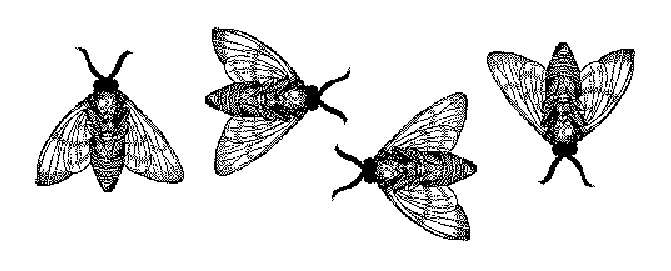
\includegraphics{flies}
% \caption{A sample black and white graphic
% that needs to span two columns of text.}
% \end{figure*}
%
%
% \begin{figure}
% 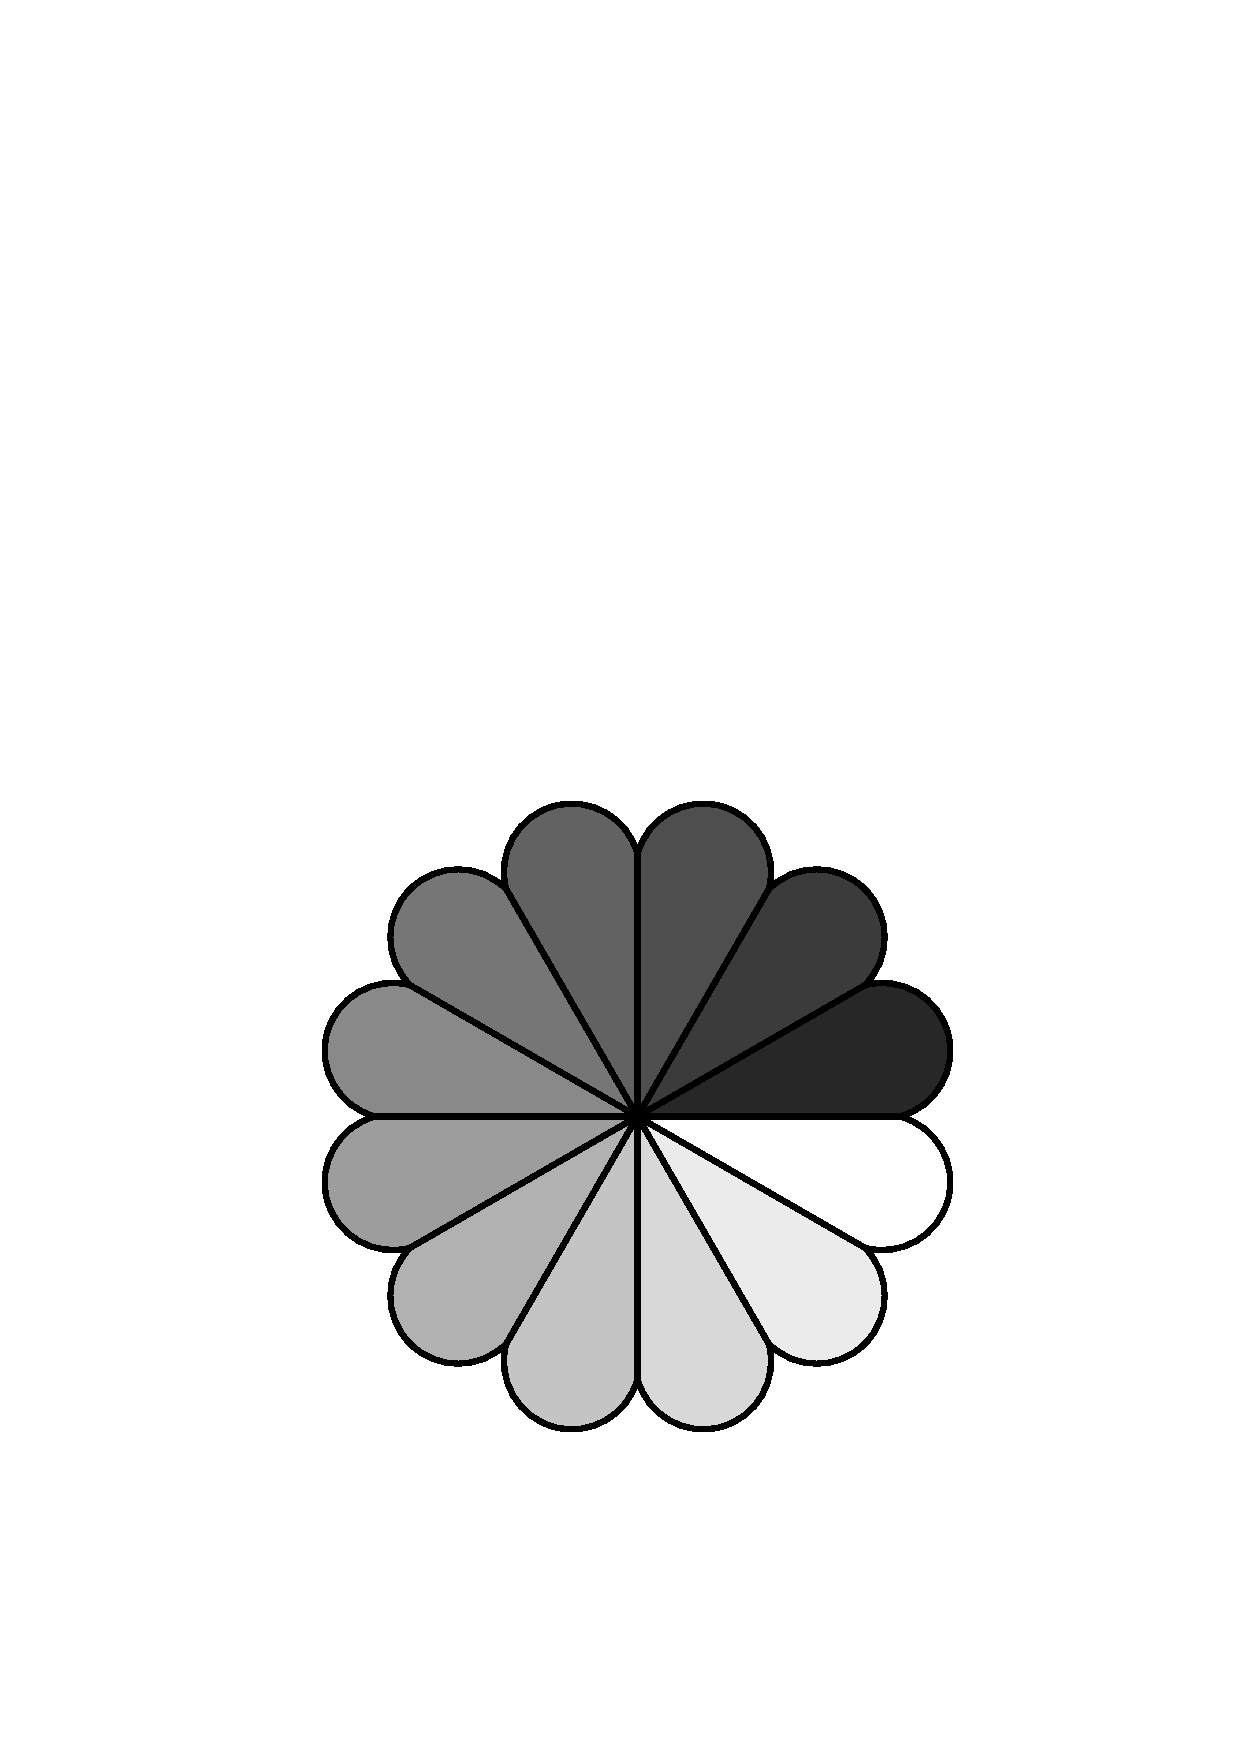
\includegraphics[height=1in, width=1in]{rosette}
% \caption{A sample black and white graphic that has
% been resized with the \texttt{includegraphics} command.}
% \end{figure}
%
% \subsection{Theorem-like Constructs}
%
% Other common constructs that may occur in your article are the forms
% for logical constructs like theorems, axioms, corollaries and proofs.
% ACM uses two types of these constructs:  theorem-like and
% definition-like.
%
% Here is a theorem:
% \begin{theorem}
%   Let $f$ be continuous on $[a,b]$.  If $G$ is
%   an antiderivative for $f$ on $[a,b]$, then
%   \begin{displaymath}
%     \int^b_af(t)\,dt = G(b) - G(a).
%   \end{displaymath}
% \end{theorem}
%
% Here is a definition:
% \begin{definition}
%   If $z$ is irrational, then by $e^z$ we mean the
%   unique number that has
%   logarithm $z$:
%   \begin{displaymath}
%     \log e^z = z.
%   \end{displaymath}
% \end{definition}
%
% The pre-defined theorem-like constructs are \textbf{theorem},
% \textbf{conjecture}, \textbf{proposition}, \textbf{lemma} and
% \textbf{corollary}.  The pre-defined de\-fi\-ni\-ti\-on-like constructs are
% \textbf{example} and \textbf{definition}.  You can add your own
% constructs using the \textsl{amsthm} interface~\cite{Amsthm15}.  The
% styles used in the \verb|\theoremstyle| command are \textbf{acmplain}
% and \textbf{acmdefinition}.
%
% Another construct is \textbf{proof}, for example,
%
% \begin{proof}
%   Suppose on the contrary there exists a real number $L$ such that
%   \begin{displaymath}
%     \lim_{x\rightarrow\infty} \frac{f(x)}{g(x)} = L.
%   \end{displaymath}
%   Then
%   \begin{displaymath}
%     l=\lim_{x\rightarrow c} f(x)
%     = \lim_{x\rightarrow c}
%     \left[ g{x} \cdot \frac{f(x)}{g(x)} \right ]
%     = \lim_{x\rightarrow c} g(x) \cdot \lim_{x\rightarrow c}
%     \frac{f(x)}{g(x)} = 0\cdot L = 0,
%   \end{displaymath}
%   which contradicts our assumption that $l\neq 0$.
% \end{proof}

\section{Conclusions}
This paragraph will end the body of this sample document.
Remember that you might still have Acknowledgments or
Appendices; brief samples of these
follow.  There is still the Bibliography to deal with; and
we will make a disclaimer about that here: with the exception
of the reference to the \LaTeX\ book, the citations in
this paper are to articles which have nothing to
do with the present subject and are used as
examples only.
%\end{document}  % This is where a 'short' article might terminate



\appendix
%Appendix A
\section{Headings in Appendices}
The rules about hierarchical headings discussed above for
the body of the article are different in the appendices.
In the \textbf{appendix} environment, the command
\textbf{section} is used to
indicate the start of each Appendix, with alphabetic order
designation (i.e., the first is A, the second B, etc.) and
a title (if you include one).  So, if you need
hierarchical structure
\textit{within} an Appendix, start with \textbf{subsection} as the
highest level. Here is an outline of the body of this
document in Appendix-appropriate form:
\subsection{Introduction}
\subsection{The Body of the Paper}
\subsubsection{Type Changes and  Special Characters}
\subsubsection{Math Equations}
\paragraph{Inline (In-text) Equations}
\paragraph{Display Equations}
\subsubsection{Citations}
\subsubsection{Tables}
\subsubsection{Figures}
\subsubsection{Theorem-like Constructs}
\subsubsection*{A Caveat for the \TeX\ Expert}
\subsection{Conclusions}
\subsection{References}
Generated by bibtex from your \texttt{.bib} file.  Run latex,
then bibtex, then latex twice (to resolve references)
to create the \texttt{.bbl} file.  Insert that \texttt{.bbl}
file into the \texttt{.tex} source file and comment out
the command \texttt{{\char'134}thebibliography}.
% This next section command marks the start of
% Appendix B, and does not continue the present hierarchy
\section{More Help for the Hardy}

Of course, reading the source code is always useful.  The file
\path{acmart.pdf} contains both the user guide and the commented
code.

\begin{acks}
  The authors would like to thank Dr. Yuhua Li for providing the
  matlab code of  the \textit{BEPS} method.

  The authors would also like to thank the anonymous referees for
  their valuable comments and helpful suggestions. The work is
  supported by the \grantsponsor{GS501100001809}{National Natural
    Science Foundation of
    China}{http://dx.doi.org/10.13039/501100001809} under Grant
  No.:~\grantnum{GS501100001809}{61273304}
  and~\grantnum[http://www.nnsf.cn/youngscientsts]{GS501100001809}{Young
    Scientsts' Support Program}.

\end{acks}
